% Created 2025-06-30 Mon 15:39
% Intended LaTeX compiler: pdflatex
\documentclass[bigger,aspectratio=169]{beamer}
  \usepackage{caption, subcaption, csquotes, amssymb, xcolor}
\usepackage[english]{babel}
\titlegraphic{\includesvg[height=1cm]{./figs/IE_Unicamp}\hspace*{1.25cm}\includesvg[height=1cm]{./figs/SSSA}\hspace*{1.25cm} \includesvg[height=1cm]{./figs/YSI}}
\AtBeginSection[]{
\begin{frame}{Outline}
\tableofcontents[currentsection]
\end{frame}
}
\usepackage[utf8]{inputenc}
\usepackage[T1]{fontenc}
\usepackage{amsmath}
\usepackage{amsfonts}
\usepackage{amssymb}
\usepackage{multicol}
\usepackage{graphicx}
\usepackage{textpos}
\usepackage{caption}
\usepackage{subfig}
\usepackage{svg}
\usepackage{pgfpages}
\usepackage{epstopdf}
\epstopdfsetup{update} % only regenerate if changed
\DeclareGraphicsRule{.eps}{pdf}{.pdf}{`epstopdf #1}
\usepackage{tikz}
\usetikzlibrary{arrows.meta, positioning, shapes}
\usepackage{fontawesome5}
\usetheme{metropolis}
\usecolortheme{beaver}
\author{Gabriel Petrini}
\date{July, 2025}
\title{ABM Macro Lab: Agent-based Modelling Tools}
\subtitle{Session 01}
\hypersetup{
 pdfauthor={Gabriel Petrini},
 pdftitle={ABM Macro Lab: Agent-based Modelling Tools},
 pdfkeywords={},
 pdfsubject={},
 pdfcreator={Emacs 29.3 (Org mode 9.7.31)}, 
 pdflang={English}}

% Setup for code blocks [1/2]

\usepackage{fvextra}

\fvset{%
  commandchars=\\\{\},
  highlightcolor=white!95!black!80!blue,
  breaklines=true,
  breaksymbol=\color{white!60!black}\tiny\ensuremath{\hookrightarrow}}

% Make line numbers smaller and grey.
\renewcommand\theFancyVerbLine{\footnotesize\color{black!40!white}\arabic{FancyVerbLine}}

\usepackage{xcolor}

% In case engrave-faces-latex-gen-preamble has not been run.
\providecolor{EfD}{HTML}{f7f7f7}
\providecolor{EFD}{HTML}{28292e}

% Define a Code environment to prettily wrap the fontified code.
\usepackage[breakable,xparse]{tcolorbox}
\DeclareTColorBox[]{Code}{o}%
{colback=EfD!98!EFD, colframe=EfD!95!EFD,
  fontupper=\footnotesize\setlength{\fboxsep}{0pt},
  colupper=EFD,
  IfNoValueTF={#1}%
  {boxsep=2pt, arc=2.5pt, outer arc=2.5pt,
    boxrule=0.5pt, left=2pt}%
  {boxsep=2.5pt, arc=0pt, outer arc=0pt,
    boxrule=0pt, leftrule=1.5pt, left=0.5pt},
  right=2pt, top=1pt, bottom=0.5pt,
  breakable}

% Support listings with captions
\usepackage{float}
\floatstyle{plain}
\newfloat{listing}{htbp}{lst}
\newcommand{\listingsname}{Listing}
\floatname{listing}{\listingsname}
\newcommand{\listoflistingsname}{List of Listings}
\providecommand{\listoflistings}{\listof{listing}{\listoflistingsname}}


% Setup for code blocks [2/2]: syntax highlighting colors

\newcommand\efstrut{\vrule height 2.1ex depth 0.8ex width 0pt}
\definecolor{EFD}{HTML}{383a42}
\definecolor{EfD}{HTML}{fafafa}
\newcommand{\EFD}[1]{\textcolor{EFD}{#1}} % default
\newcommand{\EFvp}[1]{#1} % variable-pitch
\definecolor{EFh}{HTML}{9ca0a4}
\newcommand{\EFh}[1]{\textcolor{EFh}{#1}} % shadow
\definecolor{EFsc}{HTML}{50a14f}
\newcommand{\EFsc}[1]{\textcolor{EFsc}{#1}} % success
\definecolor{EFw}{HTML}{986801}
\newcommand{\EFw}[1]{\textcolor{EFw}{#1}} % warning
\definecolor{EFe}{HTML}{e45649}
\newcommand{\EFe}[1]{\textcolor{EFe}{#1}} % error
\definecolor{Efl}{HTML}{c6c7c7}
\newcommand{\EFl}[1]{\colorbox{Efl}{\efstrut{}\textbf{#1}}} % link
\definecolor{EFlv}{HTML}{8b008b}
\definecolor{Eflv}{HTML}{c6c7c7}
\newcommand{\EFlv}[1]{\colorbox{Eflv}{\efstrut{}\textcolor{EFlv}{\textbf{#1}}}} % link-visited
\definecolor{EFhi}{HTML}{f0f0f0}
\definecolor{Efhi}{HTML}{4078f2}
\newcommand{\EFhi}[1]{\colorbox{Efhi}{\efstrut{}\textcolor{EFhi}{#1}}} % highlight
\definecolor{EFc}{HTML}{9ca0a4}
\newcommand{\EFc}[1]{\textcolor{EFc}{#1}} % font-lock-comment-face
\definecolor{EFcd}{HTML}{9ca0a4}
\newcommand{\EFcd}[1]{\textcolor{EFcd}{#1}} % font-lock-comment-delimiter-face
\definecolor{EFs}{HTML}{50a14f}
\newcommand{\EFs}[1]{\textcolor{EFs}{#1}} % font-lock-string-face
\definecolor{EFd}{HTML}{84888b}
\newcommand{\EFd}[1]{\textcolor{EFd}{\textit{#1}}} % font-lock-doc-face
\definecolor{EFm}{HTML}{b751b6}
\newcommand{\EFm}[1]{\textcolor{EFm}{#1}} % font-lock-doc-markup-face
\definecolor{EFk}{HTML}{e45649}
\newcommand{\EFk}[1]{\textcolor{EFk}{#1}} % font-lock-keyword-face
\definecolor{EFb}{HTML}{a626a4}
\newcommand{\EFb}[1]{\textcolor{EFb}{#1}} % font-lock-builtin-face
\definecolor{EFf}{HTML}{a626a4}
\newcommand{\EFf}[1]{\textcolor{EFf}{#1}} % font-lock-function-name-face
\definecolor{EFv}{HTML}{6a1868}
\newcommand{\EFv}[1]{\textcolor{EFv}{#1}} % font-lock-variable-name-face
\definecolor{EFt}{HTML}{986801}
\newcommand{\EFt}[1]{\textcolor{EFt}{#1}} % font-lock-type-face
\definecolor{EFo}{HTML}{b751b6}
\newcommand{\EFo}[1]{\textcolor{EFo}{#1}} % font-lock-constant-face
\definecolor{EFwr}{HTML}{986801}
\newcommand{\EFwr}[1]{\textcolor{EFwr}{#1}} % font-lock-warning-face
\definecolor{EFnc}{HTML}{4078f2}
\newcommand{\EFnc}[1]{\textcolor{EFnc}{\textbf{#1}}} % font-lock-negation-char-face
\definecolor{EFpp}{HTML}{4078f2}
\newcommand{\EFpp}[1]{\textcolor{EFpp}{\textbf{#1}}} % font-lock-preprocessor-face
\definecolor{EFrc}{HTML}{4078f2}
\newcommand{\EFrc}[1]{\textcolor{EFrc}{\textbf{#1}}} % font-lock-regexp-grouping-construct
\definecolor{EFrb}{HTML}{4078f2}
\newcommand{\EFrb}[1]{\textcolor{EFrb}{\textbf{#1}}} % font-lock-regexp-grouping-backslash
\definecolor{Efob}{HTML}{e7e7e7}
\newcommand{\EFob}[1]{\colorbox{Efob}{\efstrut{}#1}} % org-block
\definecolor{Efobb}{HTML}{e7e7e7}
\newcommand{\EFobb}[1]{\colorbox{Efobb}{\efstrut{}\textit{#1}}} % org-block-begin-line
\definecolor{Efobe}{HTML}{e7e7e7}
\newcommand{\EFobe}[1]{\colorbox{Efobe}{\efstrut{}\textit{#1}}} % org-block-end-line
\definecolor{EFOa}{HTML}{e45649}
\newcommand{\EFOa}[1]{\textcolor{EFOa}{\textbf{#1}}} % outline-1
\definecolor{EFOb}{HTML}{da8548}
\newcommand{\EFOb}[1]{\textcolor{EFOb}{\textbf{#1}}} % outline-2
\definecolor{EFOc}{HTML}{b751b6}
\newcommand{\EFOc}[1]{\textcolor{EFOc}{\textbf{#1}}} % outline-3
\definecolor{EFOd}{HTML}{6f99f5}
\newcommand{\EFOd}[1]{\textcolor{EFOd}{\textbf{#1}}} % outline-4
\definecolor{EFOe}{HTML}{bc5cba}
\newcommand{\EFOe}[1]{\textcolor{EFOe}{\textbf{#1}}} % outline-5
\definecolor{EFOf}{HTML}{9fbbf8}
\newcommand{\EFOf}[1]{\textcolor{EFOf}{\textbf{#1}}} % outline-6
\definecolor{EFOg}{HTML}{d292d1}
\newcommand{\EFOg}[1]{\textcolor{EFOg}{\textbf{#1}}} % outline-7
\definecolor{EFOh}{HTML}{d8e4fc}
\newcommand{\EFOh}[1]{\textcolor{EFOh}{\textbf{#1}}} % outline-8
\newcommand{\EFhn}[1]{#1} % highlight-numbers-number
\newcommand{\EFhq}[1]{#1} % highlight-quoted-quote
\newcommand{\EFhs}[1]{#1} % highlight-quoted-symbol
\newcommand{\EFrda}[1]{#1} % rainbow-delimiters-depth-1-face
\newcommand{\EFrdb}[1]{#1} % rainbow-delimiters-depth-2-face
\newcommand{\EFrdc}[1]{#1} % rainbow-delimiters-depth-3-face
\newcommand{\EFrdd}[1]{#1} % rainbow-delimiters-depth-4-face
\newcommand{\EFrde}[1]{#1} % rainbow-delimiters-depth-5-face
\newcommand{\EFrdf}[1]{#1} % rainbow-delimiters-depth-6-face
\newcommand{\EFrdg}[1]{#1} % rainbow-delimiters-depth-7-face
\newcommand{\EFrdh}[1]{#1} % rainbow-delimiters-depth-8-face
\newcommand{\EFrdi}[1]{#1} % rainbow-delimiters-depth-9-face
\definecolor{EFany}{HTML}{986801}
\definecolor{Efany}{HTML}{986801}
\newcommand{\EFany}[1]{\colorbox{Efany}{\efstrut{}\textcolor{EFany}{#1}}} % ansi-color-yellow
\definecolor{EFanr}{HTML}{e45649}
\definecolor{Efanr}{HTML}{e45649}
\newcommand{\EFanr}[1]{\colorbox{Efanr}{\efstrut{}\textcolor{EFanr}{#1}}} % ansi-color-red
\definecolor{EFanb}{HTML}{fafafa}
\newcommand{\EFanb}[1]{\textcolor{EFanb}{#1}} % ansi-color-black
\definecolor{EFang}{HTML}{50a14f}
\definecolor{Efang}{HTML}{50a14f}
\newcommand{\EFang}[1]{\colorbox{Efang}{\efstrut{}\textcolor{EFang}{#1}}} % ansi-color-green
\definecolor{EFanB}{HTML}{4078f2}
\definecolor{EfanB}{HTML}{4078f2}
\newcommand{\EFanB}[1]{\colorbox{EfanB}{\efstrut{}\textcolor{EFanB}{#1}}} % ansi-color-blue
\definecolor{EFanc}{HTML}{0184bc}
\definecolor{Efanc}{HTML}{0184bc}
\newcommand{\EFanc}[1]{\colorbox{Efanc}{\efstrut{}\textcolor{EFanc}{#1}}} % ansi-color-cyan
\definecolor{Efanw}{HTML}{383a42}
\newcommand{\EFanw}[1]{\colorbox{Efanw}{\efstrut{}#1}} % ansi-color-white
\definecolor{EFanm}{HTML}{a626a4}
\definecolor{Efanm}{HTML}{a626a4}
\newcommand{\EFanm}[1]{\colorbox{Efanm}{\efstrut{}\textcolor{EFanm}{#1}}} % ansi-color-magenta
\definecolor{EFANy}{HTML}{a77e27}
\definecolor{EfANy}{HTML}{a77e27}
\newcommand{\EFANy}[1]{\colorbox{EfANy}{\efstrut{}\textcolor{EFANy}{#1}}} % ansi-color-bright-yellow
\definecolor{EFANr}{HTML}{e86f64}
\definecolor{EfANr}{HTML}{e86f64}
\newcommand{\EFANr}[1]{\colorbox{EfANr}{\efstrut{}\textcolor{EFANr}{#1}}} % ansi-color-bright-red
\definecolor{EFANb}{HTML}{9ca0a4}
\definecolor{EfANb}{HTML}{9ca0a4}
\newcommand{\EFANb}[1]{\colorbox{EfANb}{\efstrut{}\textcolor{EFANb}{#1}}} % ansi-color-bright-black
\definecolor{EFANg}{HTML}{6aaf69}
\definecolor{EfANg}{HTML}{6aaf69}
\newcommand{\EFANg}[1]{\colorbox{EfANg}{\efstrut{}\textcolor{EFANg}{#1}}} % ansi-color-bright-green
\definecolor{EFANB}{HTML}{5c8cf3}
\definecolor{EfANB}{HTML}{5c8cf3}
\newcommand{\EFANB}[1]{\colorbox{EfANB}{\efstrut{}\textcolor{EFANB}{#1}}} % ansi-color-bright-blue
\definecolor{EFANc}{HTML}{2796c6}
\definecolor{EfANc}{HTML}{2796c6}
\newcommand{\EFANc}[1]{\colorbox{EfANc}{\efstrut{}\textcolor{EFANc}{#1}}} % ansi-color-bright-cyan
\definecolor{EFANw}{HTML}{1b2229}
\definecolor{EfANw}{HTML}{1b2229}
\newcommand{\EFANw}[1]{\colorbox{EfANw}{\efstrut{}\textcolor{EFANw}{#1}}} % ansi-color-bright-white
\definecolor{EFANm}{HTML}{b346b1}
\definecolor{EfANm}{HTML}{b346b1}
\newcommand{\EFANm}[1]{\colorbox{EfANm}{\efstrut{}\textcolor{EFANm}{#1}}} % ansi-color-bright-magenta
\usepackage[style=authoryear]{biblatex}
\addbibresource{~/Org/zotero_refs.bib}
\begin{document}

\maketitle
\begin{frame}{Outline}
\tableofcontents
\end{frame}

\section{Introduction}
\label{sec:orge93aaec}

\begin{frame}[label={sec:orgcc5503d}]{Objectives}
Throughout the sessions, we will

\begin{enumerate}
\item Understand how LSD works.
\item Implement a chaotic model\footnote{Based on the slides of LSD manual folder}
\item Understand and implement the \textcite{dosi_2017_footprint} model on LSD
\item Analyze the model results on LSD
\end{enumerate}
\end{frame}
\begin{frame}[label={sec:orgf20f731}]{Structure of the sessions}
\begin{description}
\item[{Session 1}] Presents the general structure of LSD and perform some simulations
\item[{Session 2}] Write the industry model equations in LSD
\item[{Session 3}] Complete the scripts (if necessary), run the simulation and the analysis of results
\item[{Bonus}] A primer on sensitivity analysis
\end{description}
\end{frame}
\begin{frame}[label={sec:org9fee14a},fragile]{Repository structure}
 This presentation can be found on this \href{https://github.com/gpetrini/CodingSession}{repository} with another examples:

\url{https://github.com/gpetrini/CodingSession}

\begin{description}
\item[{Linear\_Model/fun\_linear.cpp}] Starting script for the linear model
\item[{Chaotic\_Model/fun\_chaotic.cpp}] Starting script for the chaotic model
\item[{Industry\_SummerSchool/fun\_industry.cpp}] Starting script for the industry model
\item[{Sim*.lsd}] Are the configuration files
\end{description}

\alert{Important:} Clone/Download this folder under \texttt{LSD/Work/}
\begin{block}{Missed something?}
\texttt{*\_complete.cpp} contains the complete equation file for reference.
\end{block}
\end{frame}
\section{Crash course on LSD}
\label{sec:org3fb6557}

\begin{frame}[label={sec:org0dbdc35},fragile]{C++ for LSD I}
 LSD adds macros to \texttt{C++}.
As a consequence, some basic knowledge on \texttt{C++} is usefull.
What do we need to know here?
\begin{columns}
\begin{column}{0.4\columnwidth}
\begin{block}{In python, R}
\begin{Code}
\begin{Verbatim}
\color{EFD}\EFv{x} = 5 \EFcd{\#} \EFc{A comment}
\EFv{y} = 2.5
\EFcd{\#\#} \EFc{We do not need to}
\EFcd{\#\#} \EFc{work with pointers}
\end{Verbatim}
\end{Code}
\end{block}
\end{column}
\begin{column}{0.4\columnwidth}
\begin{block}{In C++}
\begin{Code}
\begin{Verbatim}
\color{EFD}\EFt{int} \EFv{x} = 5; \EFcd{//} \EFc{A comment}
\EFt{double} \EFv{y} = 2.5;
\EFt{object} *\EFv{agent}; \EFcd{//} \EFc{Latter}
\end{Verbatim}
\end{Code}
\end{block}
\end{column}
\end{columns}
\begin{block}{Compilation}
Different from python and R, we need to \alert{compile} our code before using it.
\end{block}
\end{frame}
\begin{frame}[label={sec:orgaae6dfa},fragile]{C++ for LSD II}
 To avoid initializing everything, LSD has some already initialized variables:

\begin{Code}
\begin{Verbatim}
\color{EFD}v[0] = 10; \EFcd{//} \EFc{We can assing number to}
v[1] = 50; \EFcd{//} \EFc{a vector (always available)}
T; \EFcd{//} \EFc{Current simulation time}
i = 1; \EFcd{//} \EFc{i,h,j,k can be used for integers}
cur; cur1; \EFcd{//} \EFc{Pre-allocated pointers}
\end{Verbatim}
\end{Code}

Those are \alert{local variables} that we can use on equations.
\begin{block}{Debbuging}
LSD has an internal debbuger that allow us to look to local variables on the fly.
\end{block}
\end{frame}
\begin{frame}[label={sec:org88ba2e7},fragile]{Macros I}
 \begin{figure}[htbp]
\centering
\includegraphics[width=.9\linewidth]{./figs/Macros_LSD.pdf}
\caption{\label{}General structure of most LSD macros}
\end{figure}

\begin{itemize}
\item \Verb[commandchars=\\\{\},highlightcolor=white!95!black!80!blue,breaklines=true,breaksymbol=\color{white!60!black}\tiny\ensuremath{\hookrightarrow}]{\color{EFD}\EFo{VLS}(\EFo{POS}, \EFs{"NAME"}, 1)} Returns the value of \texttt{NAME} at lag \texttt{1}, position \texttt{POS}
\item \Verb[commandchars=\\\{\},highlightcolor=white!95!black!80!blue,breaklines=true,breaksymbol=\color{white!60!black}\tiny\ensuremath{\hookrightarrow}]{\color{EFD}\EFo{SUMS}(\EFo{POS}, \EFs{"NAME"})} Sums the value of variable \texttt{NAME} at position \texttt{POS}
\item \Verb[commandchars=\\\{\},highlightcolor=white!95!black!80!blue,breaklines=true,breaksymbol=\color{white!60!black}\tiny\ensuremath{\hookrightarrow}]{\color{EFD}\EFo{SEARCHS}(\EFo{PARENT}, \EFs{"AGT"})} Searches for agent \texttt{AGT} starting from \texttt{PARENT}
\item \Verb[commandchars=\\\{\},highlightcolor=white!95!black!80!blue,breaklines=true,breaksymbol=\color{white!60!black}\tiny\ensuremath{\hookrightarrow}]{\color{EFD}\EFo{WRITELS}(\EFo{POS}, \EFs{"NAME"}, 1)} Overwrites \texttt{NAME} at lag \texttt{1} at position \texttt{POS}
\end{itemize}
\end{frame}
\begin{frame}[label={sec:org2e95eee}]{Macros II}
\begin{figure}[htbp]
\centering
\includegraphics[width=.9\linewidth]{figs/LSD_Macros_ScreenShot.png}
\caption{Other LSD macros}
\end{figure}
\end{frame}
\begin{frame}[label={sec:orgdb66af1},fragile]{Macro example I}
 How can we write the following equation using LSD syntax?
\[X_{t} = X_{t-1} + m\]
\begin{Code}
\begin{Verbatim}
\color{EFD}\EFo{EQUATION}(\EFs{"X"}) \EFcd{//} \EFc{This is a single-line comment}
\EFcd{/*}
\EFc{This is a multi-line comment}
\EFcd{*/}
v[0] = VL(\EFs{"X"},1); \EFcd{//}\EFc{past value of X, lagged of 1 period}
v[1] = V(\EFs{"m"}); \EFcd{//}\EFc{current value of m (variable or parameter)}
v[2] = v[0] + v[1]; \EFcd{//} \EFc{v[n] are local variables}
\EFo{RESULT}(v[2]) \EFcd{//} \EFc{Specify the output of the function}
\end{Verbatim}
\end{Code}
\begin{block}{Variable or parameter?}
As a rule of thumb, variables have an \texttt{EQUATION} associated, parameters do not.
\end{block}
\end{frame}
\begin{frame}[label={sec:orgb75681d},fragile]{Macro example II}
 How can we write the following equation using LSD syntax?

\[Y_{t} = \sum_{i=1}^{n} X_{n,t} + W_{n,t-1}\]



\begin{Code}
\begin{Verbatim}
\color{EFD}\EFo{EQUATION}(\EFs{"Y"})
v[0] = 0; \EFcd{//} \EFc{Initialize the Accumulation}
\EFv{CYCLE}(cur, \EFs{"Firm"}) \{ \EFcd{//} \EFc{Similar to a for-loop in other languages}
    v[1] = VS(cur, \EFs{"X"}); \EFcd{//} \EFc{cur points to a "Firm" object}
    v[2] = \EFo{VLS}(cur, \EFs{"W"}, 1); \EFcd{//} \EFc{cur is a locally defined pointer}
    v[3] = v[1] + v[2];
    v[0] = v[0] + v[3];
\}
\EFo{RESULT}(v[0])
\end{Verbatim}
\end{Code}
\end{frame}
\begin{frame}[label={sec:org68133e4},fragile]{Macro example III}
 We can also write on an alternative way

\[Y_{t} = \sum_{i=1}^{n} X_{n,t} + W_{n,t-1}\]



\begin{Code}
\begin{Verbatim}
\color{EFD}\EFo{EQUATION}(\EFs{"Y"})
\EFcd{//} \EFc{If X and W are bellow Y on the tree (later)}
v[0] = \EFo{SUM}(\EFs{"X"});
v[1] = \EFo{SUML}(\EFs{"W"}, 1);
v[2] = v[0] + v[1];
\EFo{RESULT}(v[2])
\end{Verbatim}
\end{Code}
\end{frame}
\begin{frame}[label={sec:org65c426e},fragile]{Equation file}
 Any equation file (\texttt{.cpp}) must contain the following text:
\begin{Code}
\begin{Verbatim}
\color{EFD}\EFcd{//} \EFc{File created using org-mode tangle feature.}
\EFpp{\#include} \EFs{"fun\_head.h"} \EFcd{//} \EFc{This is mandatory}

\EFo{MODELBEGIN}

\EFcd{//} \EFc{Your code goes here}

\EFo{MODELEND}
\EFt{void} \EFf{close\_sim}(\EFt{void}) \{\}
\end{Verbatim}
\end{Code}

In our session, we will copy-and-paste the initialization equation and continue from there.
\end{frame}
\begin{frame}[label={sec:orgdeb2d04},fragile]{Model structure and data organization I}
 Besides the equation files (\texttt{.cpp} or \texttt{.h}), LSD defines the model structures on a different file (extension \texttt{.lsd}).
This special file has:

\begin{itemize}
\item Variables and parameters names
\item Model structure (where elements are)
\item Initial and parameter values
\item Simulation settings
\item Number of objects
\item Variables to plot, analyze, debug, etc
\end{itemize}
\begin{block}{LSD and OOP}
This structure ensure the modeler to think in terms of data structure.
\end{block}
\end{frame}
\section{Logistic chaotic model}
\label{sec:orgf82c075}

\begin{frame}[label={sec:orga13279c},fragile]{Start}
 Let's start with the file on \url{Chaotic\_Model/fun\_chaos.cpp}


\begin{Code}
\begin{Verbatim}
\color{EFD}\EFpp{\#include} \EFs{"fun\_head.h"} \EFcd{//} \EFc{This is mandatory}

\EFo{MODELBEGIN}

\EFcd{//} \EFc{Your code goes here}

\EFo{MODELEND}
\EFt{void} \EFf{close\_sim}(\EFt{void}) \{\}
\end{Verbatim}
\end{Code}
\end{frame}
\begin{frame}[label={sec:org4745719}]{Equation}
Consider the model made of the single equation

\[X_{t} = m\cdot X_{t-1}\cdot (1 - X_{t-1})\]

To implement this model follow this steps:
\begin{enumerate}
\item Insert the equation’s code for the model.
\item Compile and run the model (menu \alert{Model/Run}).
\item Using the Lsd model program generate one object and place in it variable \(X\) with 1 lag and parameter \(m\).
\end{enumerate}
\end{frame}
\begin{frame}[label={sec:org61fa720},fragile]{Equation on LSD}
 The model equation can be written as follows:

\[X_{t} = m\cdot X_{t-1}\cdot (1 - X_{t-1})\]

\begin{Code}
\begin{Verbatim}
\color{EFD}
\EFo{EQUATION}(\EFs{"X"})
v[0] = VL(\EFs{"X"},1);
v[1] = V(\EFs{"m"});
v[2] = v[1]*v[0]*(1-v[0]);
\EFo{RESULT}(v[2])
\end{Verbatim}
\end{Code}
\end{frame}
\begin{frame}[label={sec:org154a0f1},fragile]{Configuring the model structure}
 \begin{itemize}
\item Compile (\texttt{Model > Compile and run ...}).
\item Wait to open a new window.
\item Create a descending object called \texttt{Obj1} (\texttt{Model > Add Object})
\item Double click on \texttt{Obj1}
\item Add the Variable \(X\) (max. lags = 1, \(X_{0} = 0.5\)) and Parameter (\(m = 2\))
\item Save this configuration as \texttt{Sim1.lsd}
\item Mark \(X\) to be saved (\texttt{F5}) and run
\item Analyze the results
\end{itemize}
\end{frame}
\begin{frame}[label={sec:orga6ac1ef},fragile]{Logistic chaotic model IV}
 So far, there is nothing new if you use other programming language.
However, we can leverage from the fact that LSD is OOP.

\begin{itemize}
\item Use menu \texttt{Data/Set Number of Objects} and set to 10 the copies of \texttt{Obj1}
\item Select \(m\) and click on \texttt{Data>Initial Values ...} and set different values for each instance from \((1 \ldots 3.99)_{}\)
\item Run and plot \(X\)
\end{itemize}
\begin{block}{Key takeaways}
The source code remains untouched, while we produced a completelly different structure.
This is the benefit of isolating the code and the structure.
\end{block}
\end{frame}
\begin{frame}[label={sec:org96a401d}]{Results I}
\begin{center}
\includesvg[width=.83\linewidth]{./figs/chaos_X}
\end{center}
\end{frame}
\begin{frame}[label={sec:org313bff8}]{Sensitivity to \(m\)}
The function produces \alert{extremely} different outcomes depending on the value of \alert{\(m\)}.

\begin{itemize}
\item We will create a large number of series computed independently.
\item We will set \(m\) to a slightly different value for each series.
\item We will set the \alert{initial} points for the \(X\) to random values.
\end{itemize}
\end{frame}
\begin{frame}[label={sec:orgd722c33},fragile]{Exploiting the chaotic behaviour}
 \begin{itemize}
\item Load \texttt{Sim1.lsd} and save it as \texttt{Sim2.lsd}
\item Generate \alert{10000} copies of \texttt{Obj1}
\item Open the initial values interface with \texttt{Data/Initial Values...}
\item Use the buttons \texttt{Set All} on the side of \(m\) and \(X\) to assign values to all the elements.
\begin{itemize}
\item \(m\): \alert{Range} between 2.8 and 3.99.
\item \(X\): Random (Uniform) between 0.01 and 0.99.
\end{itemize}
\item \texttt{Run>Simulation Settings...} to set 1000 time steps.
\item Mark \(m\) to be saved
\item Save, run, analyze
\end{itemize}
\end{frame}
\begin{frame}[label={sec:orgb011e93}]{Plotting}
\begin{itemize}
\item Open Analysis of results
\item Select all \(m\) and \(X\) series
\item On the bottom right, select \alert{Cross section} and \alert{XY plot}
\item Select \alert{Points}
\item Plot for the last timestep (1000, default)
\item Hit continue and wait
\end{itemize}
\begin{block}{Key takeaways}
Once again, the code remains \alert{untouched}.
Later, we will check other features of LSD that benefit from this design principle.
\end{block}
\end{frame}
\begin{frame}[label={sec:orga33522e}]{Results II}
\begin{center}
\includesvg[width=.83\linewidth]{figs/chaotic_bifurcation}
\end{center}
\end{frame}
\section{The industry model}
\label{sec:org33815db}


\begin{frame}[label={sec:org579fbd7}]{Where are we and where are we going?}
So far, we implemented a small non-economic model.
On the following lectures, we will focus on the \alert{industry model}.

\textcite{dosi_2017_footprint} design objective: simplest industrial dynamics model capturing most \alert{stylized facts}:
\begin{itemize}
\item Persistent heterogeneity in productivity and all other performance variables
\item Persistent market share and entry-exit turbulence
\item Skewed size distributions
\item Fat-tailed distribution of growth rates
\item Scaling of the growth-variance relationship
\end{itemize}
\end{frame}
\begin{frame}[label={sec:org5e3ddac}]{Equations}
\[ \begin{array}{lrl}
\mbox{Idiosyncratic learning process:} & a_{i,t} = &a_{i,t-1}\cdot (1 + \eta\cdot\theta_{i,t})\\
\mbox{Learning shocks} & \theta_{i,t} \sim  & Beta(\beta_1, \beta_2)\\
\mbox{Market selection} & s_{i,t} =  & s_{i,t-1} \cdot \left( 1 + A\cdot\frac{a_{i,t} - \bar{a}_{t}}{\bar{a}_{t}}\right) \\
\mbox{Average productivity} & \bar{a}_{t} =  & \sum_{i=1}^{NF} s_{i, t-1}\cdot a_{i,t} \\
\mbox{Exit condition} & s_{i,t} < & s_{min}\\
\mbox{Entrant productivity} & a_{j,t} =&  \bar{a}_{t}\cdot (1 + \eta\cdot\theta_{i,t})\\
\mbox{Entrant market-share} & s_{j,t} =& 1/NF \\
\mbox{Market concentration index} & HHI_{t} =& \sum_{i=1}^{NF} (s_{i})^2 \\
\mbox{Market-share adjustment} &  s_{i} \mapsto & s_{i}\cdot \frac{1}{\sum_{i=1}^{NF} s_{i}} \Rightarrow \sum_{i=1}^{NF} s_{i} = 1 \\
\mbox{Fixed number of firms} & \#\{1, \ldots, n\} =& NF
\end{array}\]
\end{frame}
\begin{frame}[label={sec:org3721f41}]{Graph of industry model}
\resizebox{\linewidth}{!}{%
  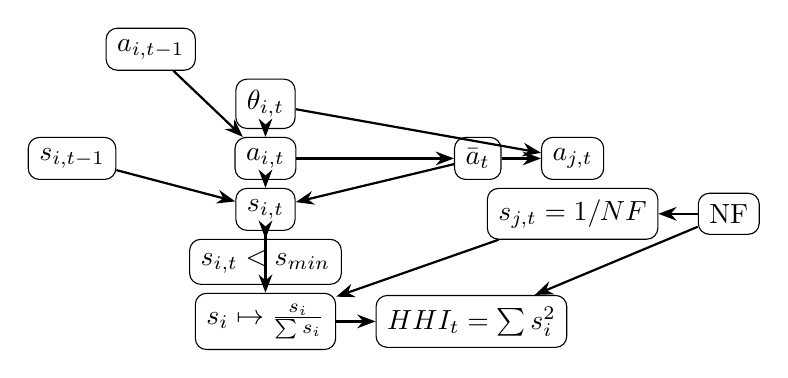
\begin{tikzpicture}[
    node distance=.1cm and 0.5cm,
    every node/.style={draw, rounded corners, minimum height=1.2em, inner sep=4pt, align=center},
    arrow/.style={-{Stealth}, thick}
    ]

    % Nodes
    \node (theta)        {$\theta_{i,t}$};
    \node (ai_tm1)       [above left=of theta] {$a_{i,t-1}$};
    \node (ai_t)         [below=of theta] {$a_{i,t}$};
    \node (si_tm1)       [left=1.5cm of ai_t] {$s_{i,t-1}$};
    \node (abar_t)       [right=2cm of ai_t] {$\bar{a}_t$};
    \node (si_t)         [below=of ai_t] {$s_{i,t}$};
    \node (exit)         [below=of si_t] {$s_{i,t} < s_{min}$};

    \node (aj_t)         [right=of abar_t] {$a_{j,t}$};
    \node (sj_t)         [below=of aj_t] {$s_{j,t} = 1/NF$};

    \node (norm_s)       [below=of exit] {$s_i \mapsto \frac{s_i}{\sum s_i}$};
    \node (HHI_t)        [right=of norm_s] {$HHI_t = \sum s_i^2$};

    \node (NF)           [right=of sj_t] {NF};

    % Arrows
    \draw[arrow] (ai_tm1) -- (ai_t);
    \draw[arrow] (theta) -- (ai_t);
    \draw[arrow] (ai_t) -- (abar_t);
    \draw[arrow] (si_tm1) -- (si_t);
    \draw[arrow] (ai_t) -- (si_t);
    \draw[arrow] (abar_t) -- (si_t);
    \draw[arrow] (si_t) -- (exit);

    \draw[arrow] (abar_t) -- (aj_t);
    \draw[arrow] (theta) -- (aj_t);
    \draw[arrow] (NF) -- (sj_t);
    \draw[arrow] (NF) -- (HHI_t);
    \draw[arrow] (si_t) -- (norm_s);
    \draw[arrow] (sj_t) -- (norm_s);
    \draw[arrow] (norm_s) -- (HHI_t);

    % Optional: Labels or braces could be added if needed
  \end{tikzpicture}
}
\end{frame}
\end{document}
